\chapter{Vývoj AI rozhraní a řešení FE issues}
\label{chap:fe_issues_ai}

Vedle hlavního projektu Importér byla významná část času věnována práci na klientských požadavcích a údržbě existujících systémů. Tato kapitola popisuje vývoj specializovaného AI modulu a řešení specifických chyb v uživatelském rozhraní.

\section{Implementace AI asistenta v prostředí AngularJS}

Jedním z nejnáročnějších úkolů byl vývoj inteligentního chatu pro specifického klienta, jehož informační systém je postaven na starší technologii \textbf{AngularJS (v1.x)} \cite{angularjs_docs}. Cílem bylo integrovat moderní jazykové modely (LLM) do tohoto prostředí a umožnit uživatelům nejen konverzaci, ale i analýzu nahraných dokumentů.

Je důležité podotknout, že framework AngularJS je v současnosti již ve fázi ukončené podpory (\textit{end-of-life}, oficiálně od 31.~12.~2021 \cite{angularjs_eol}) a v rámci standardních firemních procesů jej pro nové projekty již nenasazujeme. Volba této technologie byla v tomto případě čistě pragmatická a vynucená architekturou stávajícího informačního systému klienta. Cílem bylo vyhovět požadavku na integraci moderních funkcí do již zavedené aplikace a zajistit její další rozvoj bez nutnosti okamžité a nákladné migrace celého systému na modernější platformu.

\begin{sidewaysfigure}
    \centering
    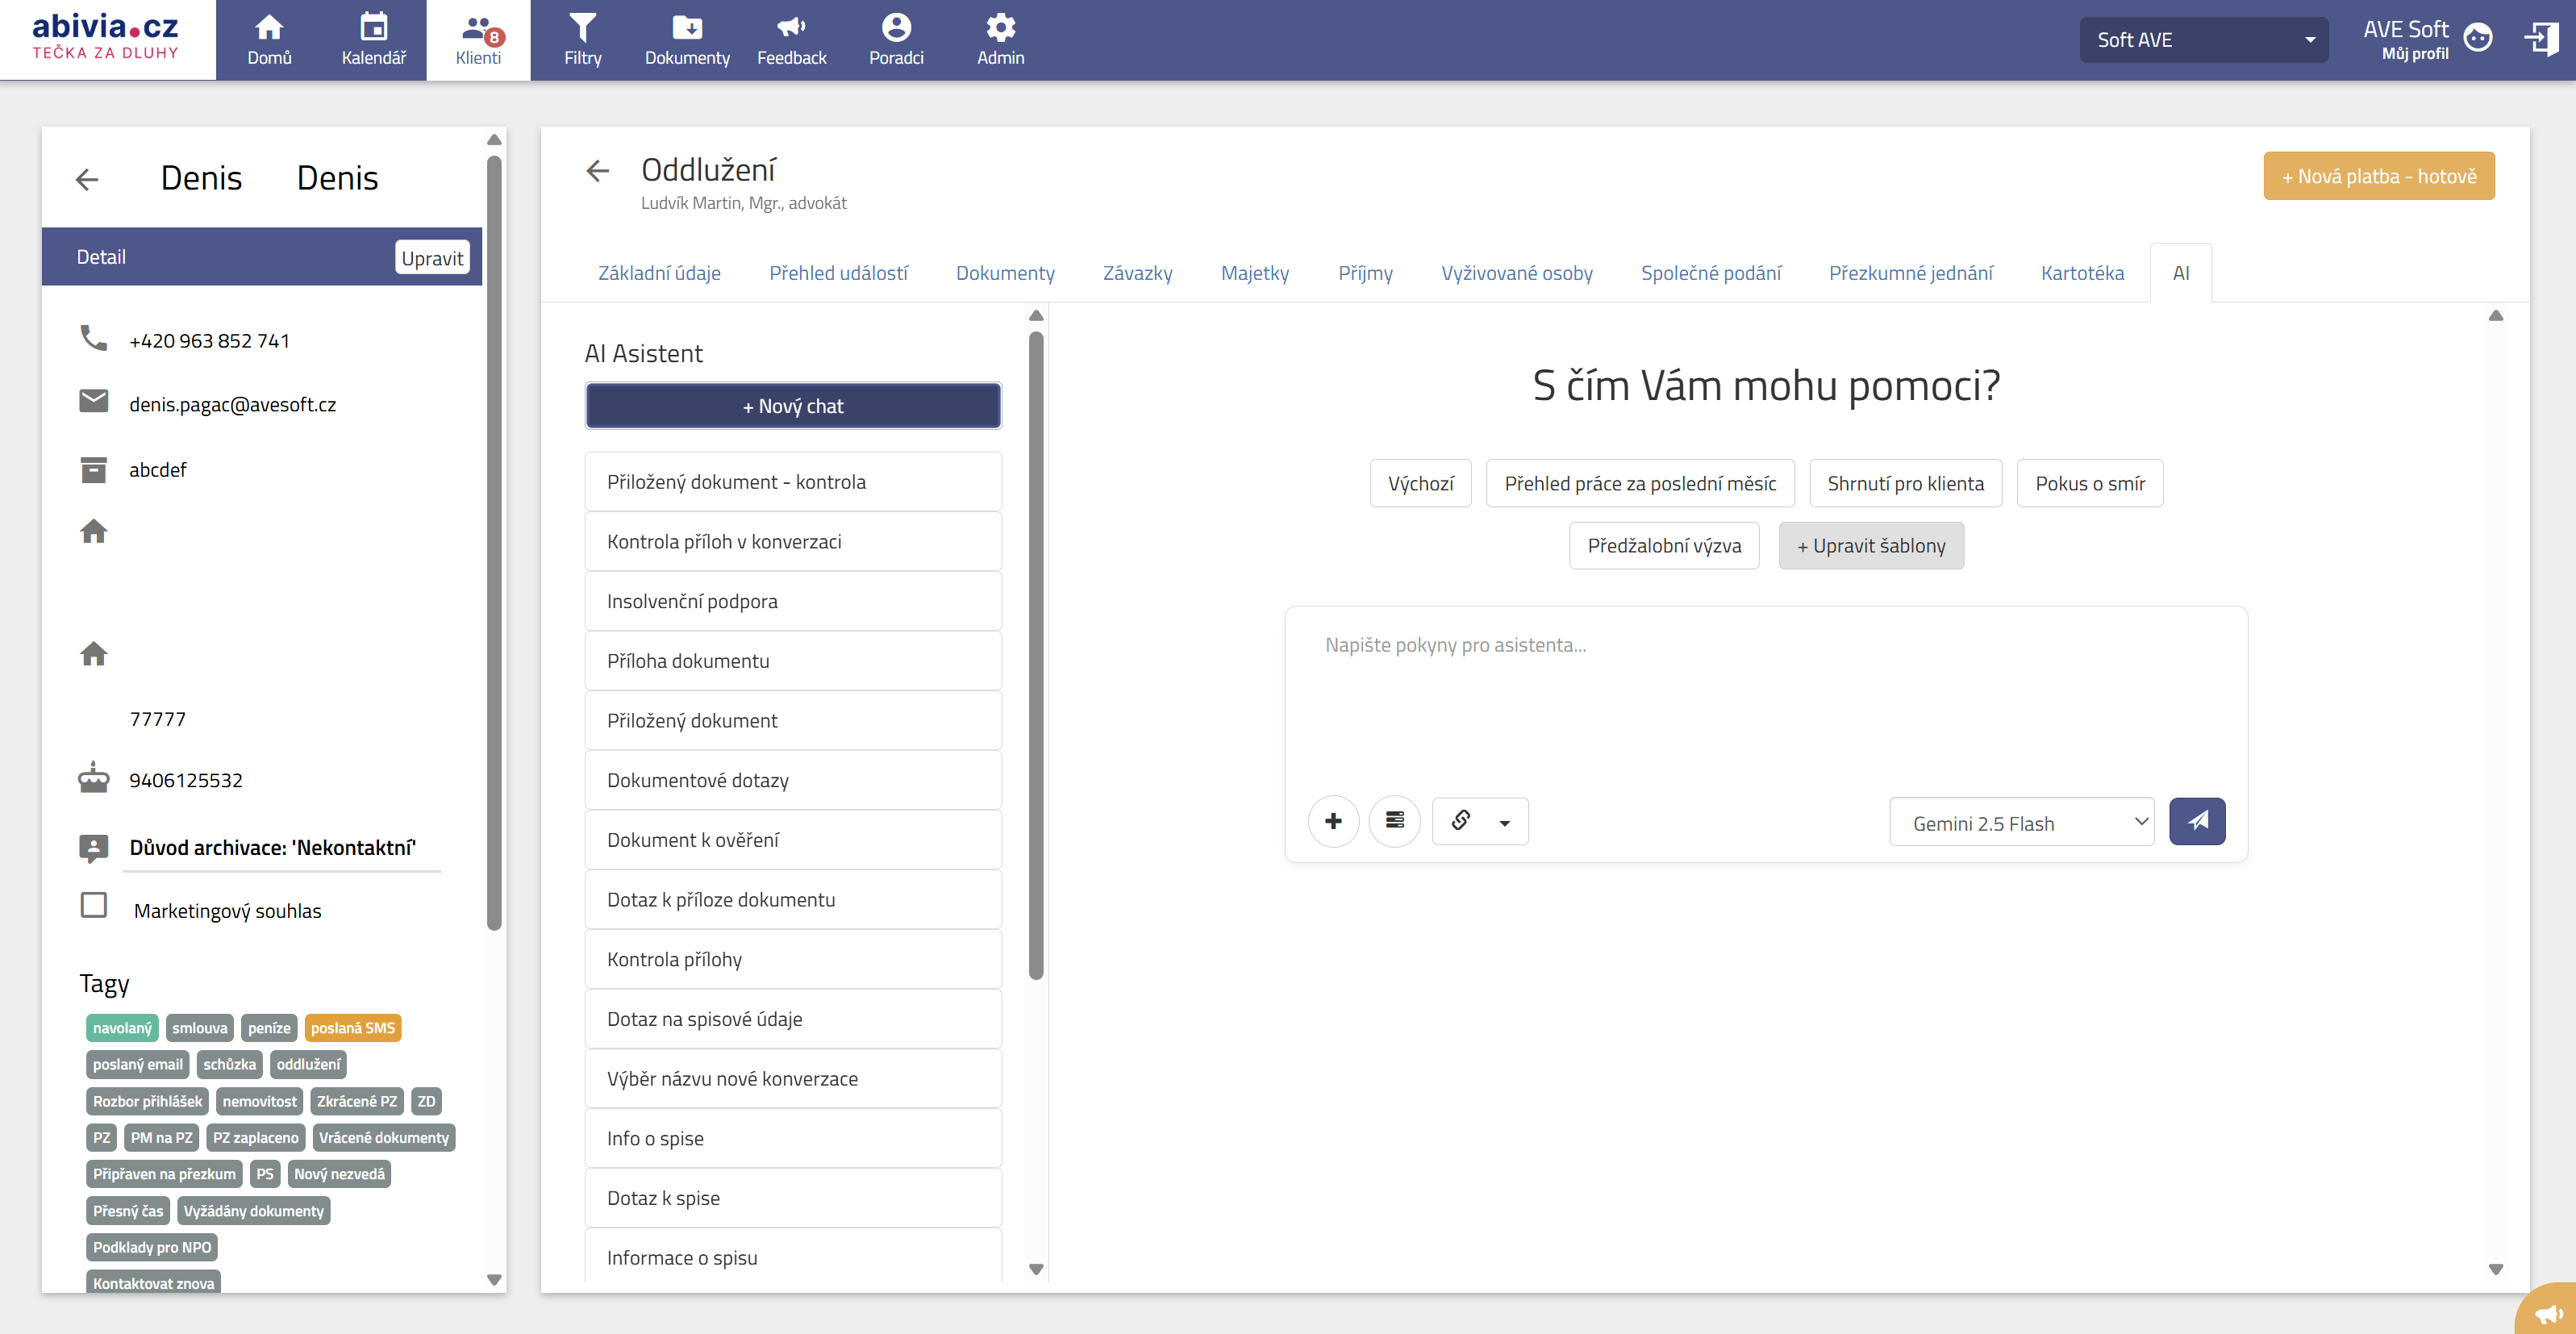
\includegraphics[width=1\textheight]{Figures/AI-new_chat.png}
    \caption{Výchozí rozhraní AI asistenta s nabídkou předdefinovaných šablon (\textit{prompt templates}) a volbou jazykového modelu}
    \label{fig:ai_templates}
\end{sidewaysfigure}

\subsection{Architektura řešení a datový tok}

Modul je rozdělen do tří vrstev, které společně zajišťují celý životní cyklus konverzace -- od odeslání dotazu až po streamování odpovědi zpět do uživatelského rozhraní. Jejich zodpovědnosti shrnuje tabulka \ref{tab:ai_layers}.

\begin{table}[H]
\centering
\caption{Vrstvy AI modulu a jejich zodpovědnosti}
\label{tab:ai_layers}
\begin{tabular}{|l|p{9cm}|}
\hline
\textbf{Vrstva} & \textbf{Zodpovědnost} \\ \hline
Prezentační (AngularJS) & Správa vláken (\textit{threads}) konverzace, rendering Markdown výstupu, upload dokumentů, sběr tokenů streamu. \\ \hline
Aplikační (C\# Service Fabric) & Orchestrace: příjem dotazu, konstrukce promptu, volání LLM API, publikace tokenů do SignalR hubu. \\ \hline
Externí LLM API & Generování odpovědi (Azure OpenAI / OpenAI \cite{openai_api}); streaming tokenů přes rozhraní Chat Completions. \\ \hline
\end{tabular}
\end{table}

Vzhledem k požadavku na plynulé zobrazování odpovědi (podobně jako v chatovacích rozhraních typu ChatGPT) nebylo možné čekat na vygenerování celé odpovědi na serveru. Řešení využívá technologii \textbf{SignalR} \cite{signalr_docs} pro real-time přenos jednotlivých tokenů textu v momentě jejich vygenerování.

Datový tok od okamžiku odeslání dotazu je následující:
\begin{enumerate}
    \item Frontend odešle HTTP POST požadavek s dotazem, identifikátorem vlákna (\texttt{partitionKey}, \texttt{rowKey}) a identifikátorem vybraného modelu (\texttt{selectedModelId}).
    \item Backendová služba \texttt{AiAgents\_Threads} dohledá konverzační vlákno v úložišti, načte jeho historii a sestaví kompletní prompt pro LLM (systémový prompt + historie zpráv + aktuální dotaz).
    \item Backend iniciuje volání Chat Completions API s parametrem \texttt{stream = true}; přijaté SSE události postupně publikuje přes SignalR hub zpět na klienta.
    \item Frontend je přihlášen k odběru události \texttt{openAIStream}; každý příchozí fragment (chunk) inkrementálně připojuje k aktuální zprávě a vynucuje překreslení UI.
    \item Po ukončení streamu backend pošle řídicí zprávu \texttt{refreshStatus = REFRESH}, která klienta informuje o dokončení a zároveň uvolní blokaci odesílacího tlačítka.
\end{enumerate}

\begin{lstlisting}[language=JavaScript, caption={Zpracování streamované odpovědi v AngularJS}]
// Naslouchání na notifikace ze SignalR hubu
hub.on('openAIStream', function(message) {
    $rootScope.$broadcast('openAIStream', message);
});

// Skládání zprávy v kontroleru (ev. zdroj: contractDetail.ts)
$scope.$on('openAIStream', function(event, chunk) {
    // Inkrementální připojení tokenu k aktuální streamované zprávě
    streamingMsg.Message += chunk;
    // Vynucení digest cyklu mimo Angular kontext
    $scope.$applyAsync();
});

// Ukončení streamu a uvolnění UI
$scope.$on('refreshStatus', function(event, status) {
    if (status === 'REFRESH') {
        $scope.isStreaming = false;
        $scope.isLoading = false;
    }
});
\end{lstlisting}

\subsection{Správa vláken konverzace a historie}

Každá konverzace je v systému reprezentována samostatným \textbf{vláknem} (\textit{thread}) identifikovaným dvojicí \texttt{partitionKey} a \texttt{rowKey} (klíče úložiště Azure Table Storage v rámci Service Fabric služby). Vlákno uchovává:
\begin{itemize}
    \item seznam všech zpráv (role \texttt{user} / \texttt{assistant}) v chronologickém pořadí,
    \item identifikátor zvoleného modelu (\texttt{idaiModel}), který je závazný pro celé vlákno,
    \item seznam vazeb na nahrané dokumenty (dokumenty se ukládají odděleně a do vlákna se připojují pouze reference).
\end{itemize}

Takto oddělené úložiště umožňuje efektivně iterovat nad historií bez nutnosti přenášet celé dokumenty, a zároveň poskytuje klientovi seznam vláken k výběru (boční panel konverzací).

Při odesílání nové zprávy frontend prostřednictvím metody \texttt{createThread()} buď pokračuje v existujícím vláknu, nebo jej nově zakládá. Výběr modelu je při prvním založení vlákna iniciálně nastaven na model označený v databázi jako výchozí (\texttt{jeVychozi = true}); uživatel jej může přepnout při vytváření vlákna, po zahájení konverzace je však model uzamčen pro zajištění konzistence odpovědí v rámci téhož vlákna.

\subsection{Zpracování nahraných dokumentů}

Klíčovým požadavkem byla analýza právních dokumentů. Tato funkce vyžadovala specifický dvoufázový proces:

\paragraph{Fáze 1 -- Upload.} Po výběru dokumentů uživatelem jsou soubory odeslány na endpoint \texttt{AiAgents\_Docs\_Upload\_ById} voláním \texttt{\$q.all()} pro paralelní zpracování. Backend každý dokument extrahuje do textové podoby (pro PDF, DOCX a obdobné formáty), uloží do trvalého úložiště a vrátí identifikátor \texttt{idDokument}. Během uploadu je UI blokováno (\texttt{uploadInProgress = true}) a odesílací tlačítko je deaktivováno.

\paragraph{Fáze 2 -- Vazba na zprávu.} Po dokončení uploadu všech souborů frontend přidá do aktuální zprávy kolekci referencí (\texttt{idDokument}, název souboru, přípona) a teprve poté zahájí samotné volání \texttt{createThread()}. Backend při sestavování promptu pro LLM načte extrahovaný obsah referencovaných dokumentů a zařadí jej do kontextového okna jazykového modelu. Tento přístup (označovaný jako \textit{in-context document loading}) je jednodušší alternativou ke vzoru Retrieval-Augmented Generation (RAG) a je vhodný pro scénáře, kde je celý dokument dostatečně malý, aby se vešel do kontextového okna modelu.

\subsection{Formátování výstupu a Markdown rendering}

Jazykové modely generují odpověď ve formátu Markdown. Pro korektní zobrazení byla nasazena knihovna \textbf{marked.js}, která v reálném čase konvertuje text na HTML. Konfigurace potlačila automatické generování ID nadpisů a mangling e-mailových adres:

\begin{lstlisting}[language=JavaScript, caption={Konfigurace Markdown parseru (marked.js)}]
const markedInstance = window.marked;
if (markedInstance && typeof markedInstance.setOptions === 'function') {
    markedInstance.setOptions({ mangle: false, headerIds: false });
}
\end{lstlisting}

Protože je rendering volán při každém tokenu, bylo nutné ošetřit i částečně dokončené bloky (např. neukončený \texttt{```} blok kódu); při nekonzistentním stavu zůstává text v surové podobě až do doručení dalšího fragmentu.

\subsection{Ošetření chybových stavů}

Streamované API přináší specifické chybové stavy, které klasické REST volání neřeší:
\begin{itemize}
    \item \textbf{Přerušení streamu na backendu} -- backend publikuje událost \texttt{openAIError}, klient uvolní UI a zobrazí informaci o selhání.
    \item \textbf{Selhání uploadu dokumentu} -- při selhání kteréhokoliv souboru je \texttt{\$q.all()} odmítnut, UI odstraní přidané zprávy a konverzace se vrátí do výchozího stavu.
    \item \textbf{Ztráta SignalR spojení} -- klient volá \texttt{signalRService.connect(contextGuid)}, který při výpadku automaticky navazuje reconnect.
\end{itemize}

\clearpage
\begin{sidewaysfigure}
    \centering
    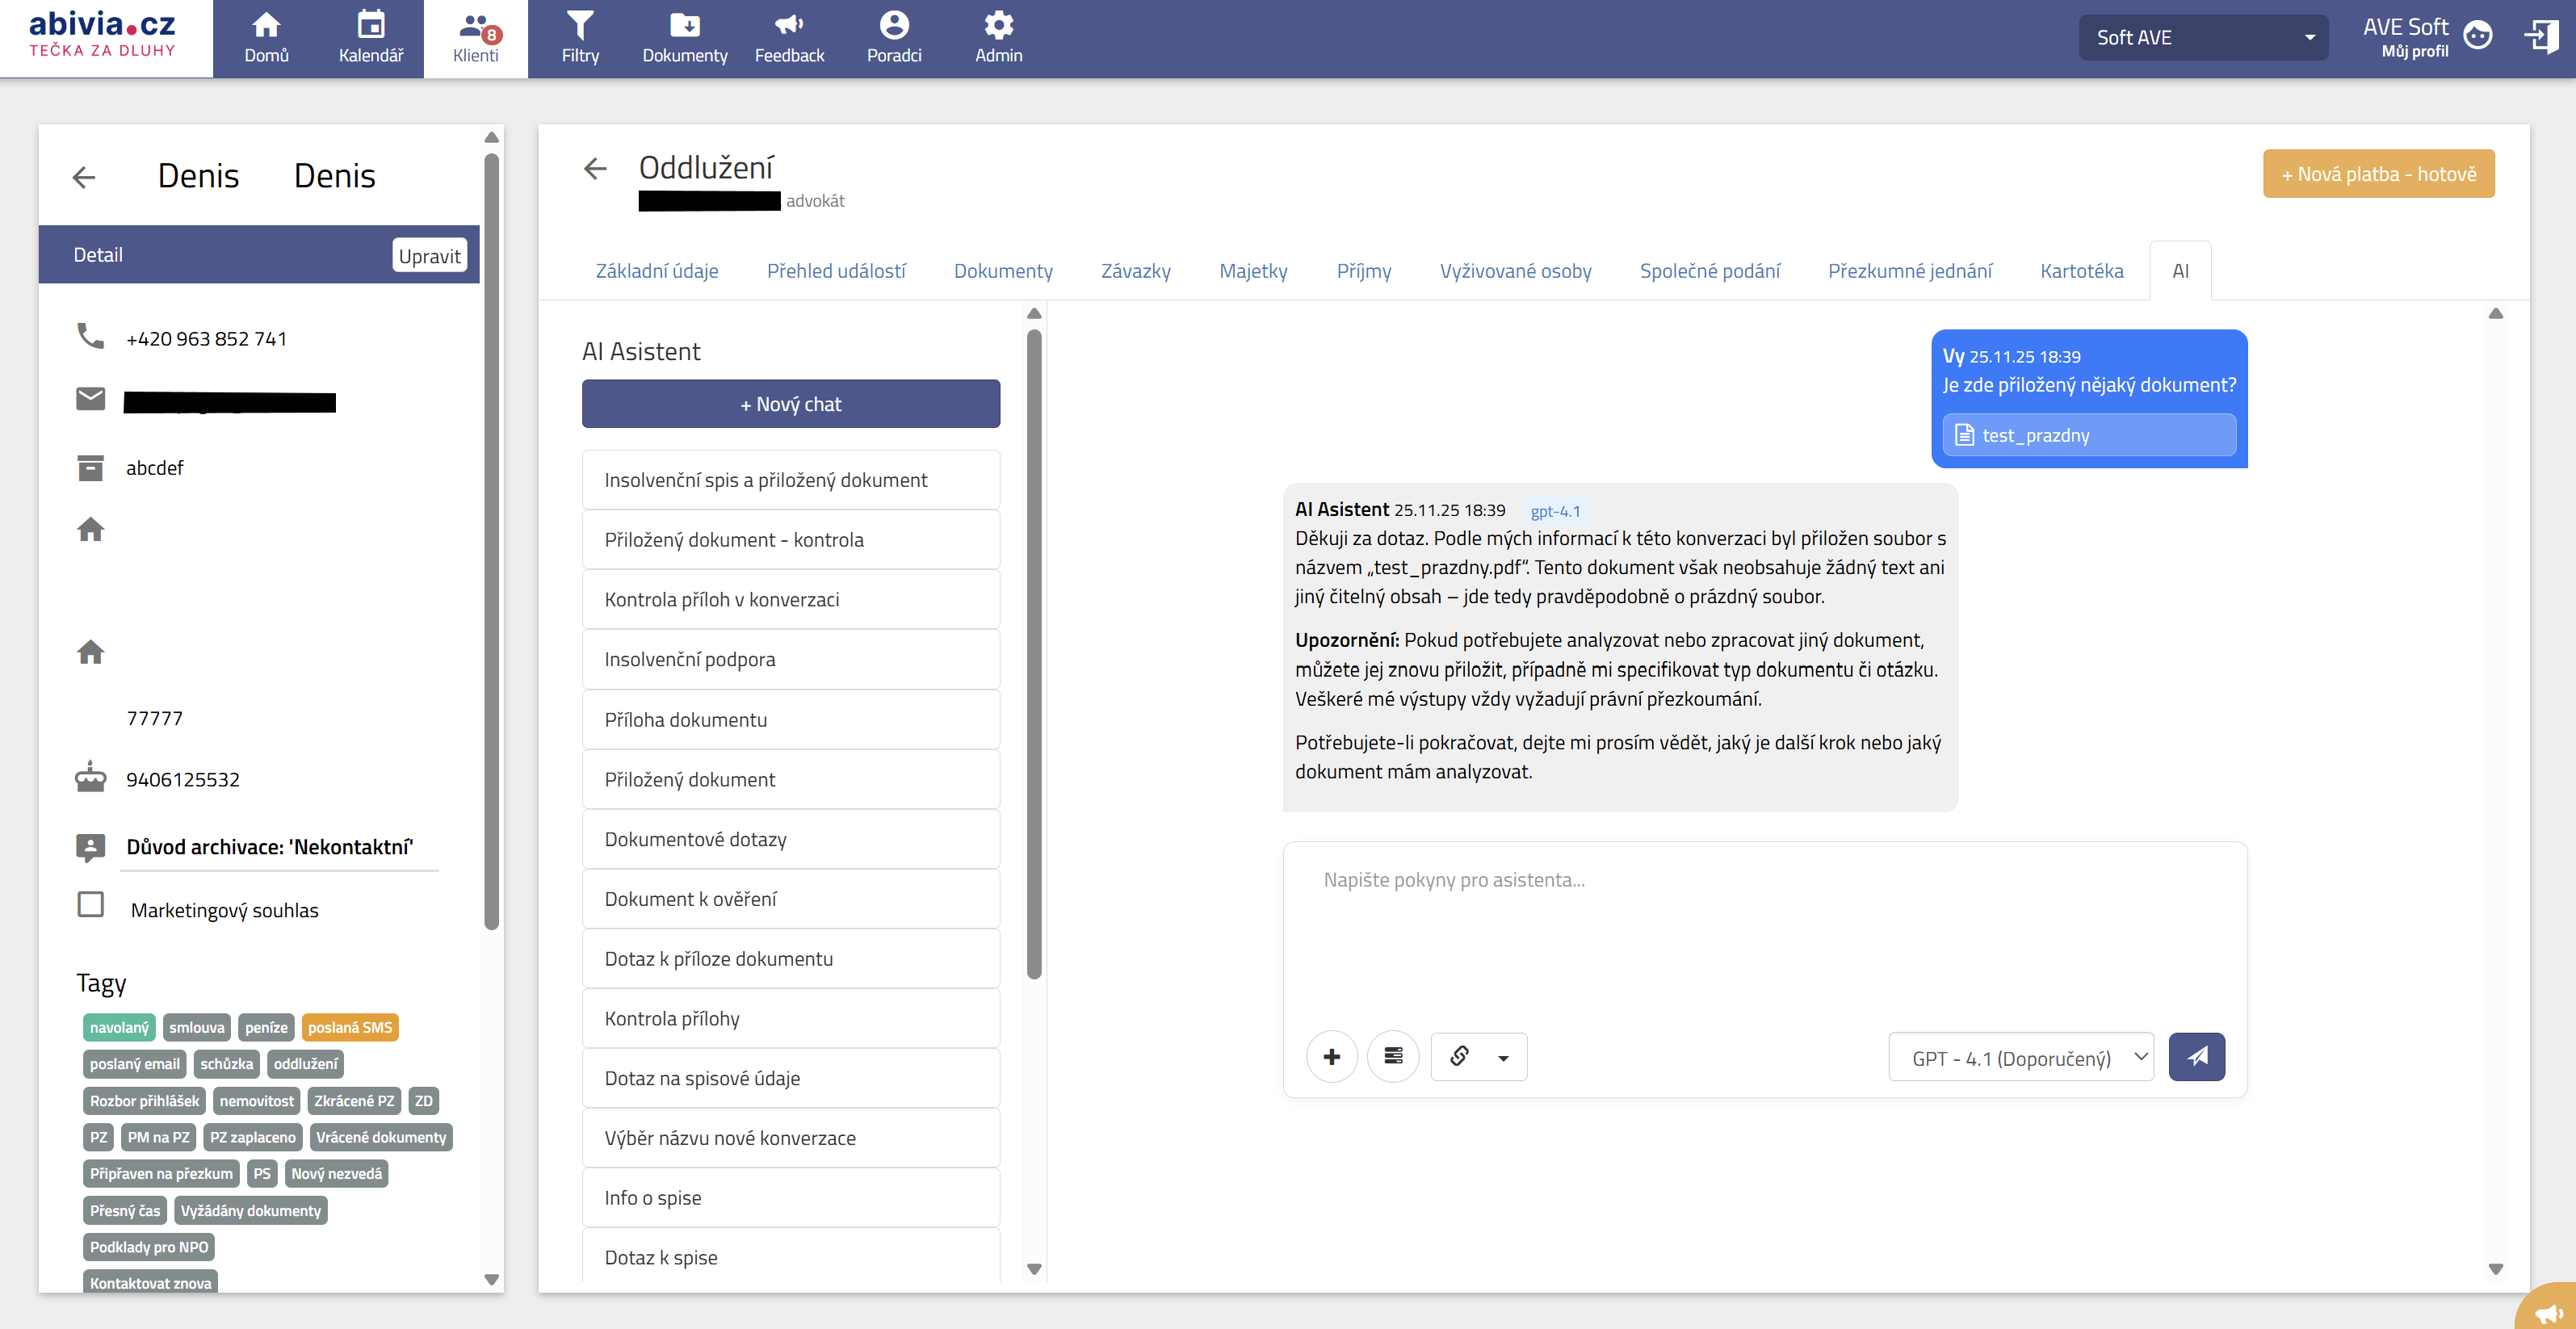
\includegraphics[width=1\textwidth]{Figures/AI-existing_chat.png}
    \caption{Ukázka probíhající konverzace s formátováním textu (Markdown) a analýzou nahraného dokumentu}
    \label{fig:ai_conversation}
\end{sidewaysfigure}
\clearpage


\section{Řešení chyb v uživatelském rozhraní (opravy chyb)}

Nedílnou součástí praxe byla analýza a opravy chyb v systému Evolio. Příkladem komplexního problému byla chyba v komponentě Přehledy (založené na knihovně DevExpress \cite{devexpress_docs}), kde docházelo k selhání načítání filtrů.

\subsection{Analýza problému: Konflikt seskupování a ukotvení}
Uživatelé hlásili, že u určitých přehledů se nenačetla data v tabulce a došlo k permanentnímu stavu načítání (spinner se nezastavil). Analýzou bylo zjištěno, že problém nastává v momentě, kdy je sloupec nastaven jako \textbf{ukotvený} (Fixed) a zároveň se podle něj \textbf{seskupuje} (Grouped).

Komponenta DevExpress v této specifické konfiguraci nedokázala správně vypočítat pozici elementů, což vedlo k chybě v konzoli a k tomu, že se data tabulky nenačetla.

\begin{figure}[H]
    \centering
    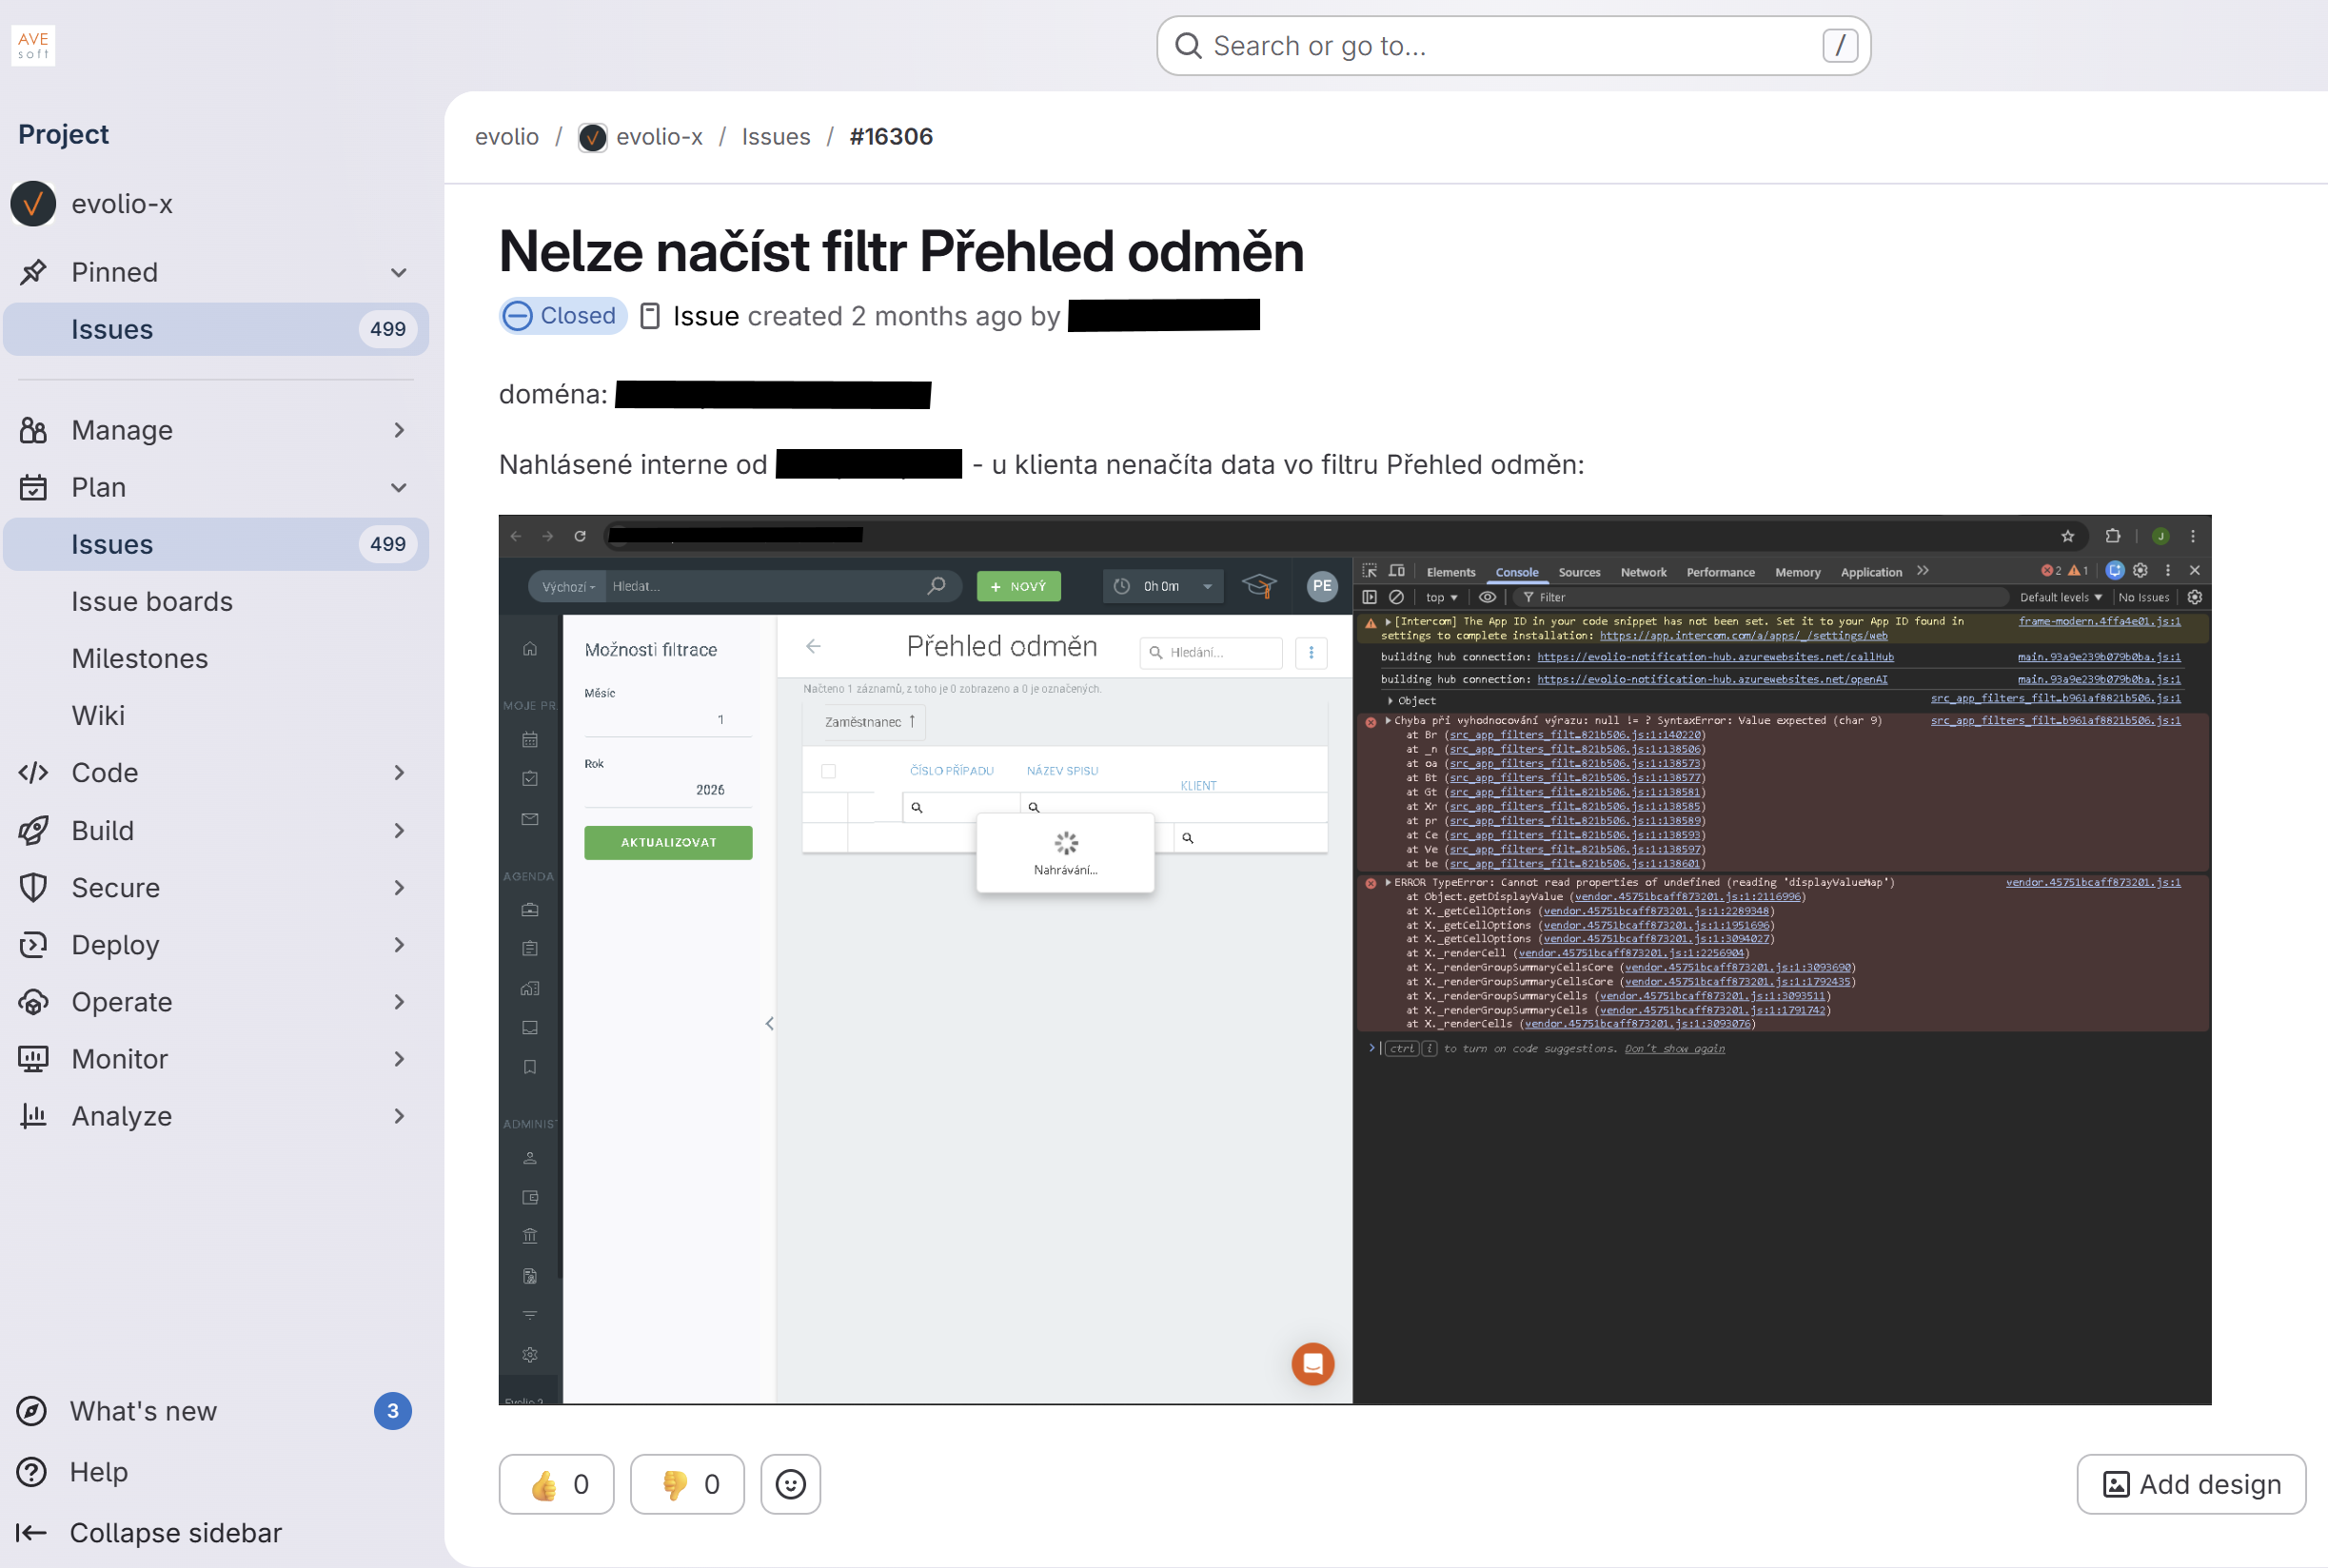
\includegraphics[width=1\textwidth]{Figures/gitlab-issue.png}
    \caption{Ukázka zadaného požadavku (issue) v systému GitLab popisující nekonzistentní chování tabulky při kombinaci Fixed + Grouped}
    \label{fig:gitlab-issue}
\end{figure}

\subsection{Implementace opravy}
Oprava spočívala v úpravě logiky, která generuje konfiguraci pro sloupce tabulky. Bylo nutné zajistit, aby se vlastnost \texttt{fixed} automaticky deaktivovala, pokud je sloupec použit pro seskupování.

\begin{lstlisting}[language=JavaScript, caption={Úprava konfigurace sloupců pro detekci konfliktu Fixed/Grouped}]
// Puvodni problematicky kod
// fixedPosition: colcf.fixed !== null ? colcf.fixed.toLowerCase() : null,
// fixed: colcf.fixed !== null,

// Nova logika s osetrenim konfliktu
const isFixed = colcf.fixed !== null &&
                colcf.fixed.toLowerCase() !== 'none' &&
                !colcf.grouped; // Klicova podminka: nesmi byt seskupeno

// Aplikace do konfigurace
const columnConfig = {
    // ... ostatni vlastnosti
    fixedPosition: isFixed ? colcf.fixed.toLowerCase() : null,
    fixed: isFixed
};
\end{lstlisting}

Tato úprava zajistila stabilitu komponenty i v případě, že uživatel (nebo uložený přehled) definoval tuto konfliktní kombinaci vlastností.
